\documentclass[12pt, letterpaper]{report}


%---------------------------------------
%Início dos pacotes
%---------------------------------------
\usepackage[margin=0.7in]{geometry} % A margem fica menor.
\usepackage[utf8]{inputenc} % Deixa os caracteres em UTF8
\usepackage{url} % Pacote para URL's.
\usepackage{hyperref} % Outro pacote para URL's.
\usepackage{graphicx} % Pacote para colocar imagens.
%---------------------------------------
%Fim dos pacotes
%---------------------------------------

\title{\Huge Guia de seguran\c{c}a para leigos} % Título do livro.
\author{Autores: Comunidade} % Autores

\begin{document} % Inicia o documento.
\maketitle % Faz o título.
\pagebreak % Termina de escrever na página.

\part{Capítulo 1 - Segurança básica}

% Espionagem em massa - Um problema mundial.
\section*{Espionagem em massa - Um problema mundial} % Coloca o título do assunto em uma nova página.

\large Um dos maiores problemas na nossa sociedade moderna é a espionagem em massa. Governos roubam os teus dados, lhe espionam e ainda dizem que é para o seu próprio bem.\\

\subsection{A espionagem governamental}

	Depois dos vazamentos (leaks) feitos por \textbf{Edward Snowden}, várias pessoas em todo o mundo passaram a se preocupar com a própria segurança e privacidade. Mas ainda assim, uma boa parcela da população não se preocupa com a própria privacidade e segurança, muitas vezes por não saber o que governos e empresas fazem com os dados coletados. Mas a população deveria sim se  preocupar com a privacidade, pois os mesmos métodos utilizado pelos governos para roubarem dados, também são utilizado por criminosos.\\

	A espionagem em massa acontece em todo e qualquer lugar do globo, não importa onde você esteja, se tem algum meio de comunicação você está vulnerável à espionagem. Mesmo que você apenas utilize um telefone fixo, você está vulnerável à espionagem.\\

\subsection{Redes sociais e os perigos à privacidade}

	Redes sociais atualmente são um dos maiores perigos para a segurança e privacidade dos usuários, visto que é possível determinar os seus gostos, seus amigos, sua família e diversas outras coisas. Sites como o Facebook, enquanto você o utiliza ele monitora o que você está acessando para poder lhe fazer propagandas direcionadas. O Google também faz isto. Embora seja a forma que estas empresas tem de ganhar dinheiro, é muito invasivo e na maioria das vezes não funciona. Mas para poder escapar desta vigilância, existem algumas coisas que podemos fazer.\\
	\begin{itemize} % Inicia a lista.
		\item Utilize as redes sociais apenas quando necessário.
		\item Sempre que for utilizar alguma rede social, utilize-a com alguma \href{https://criptowiki.miraheze.org/wiki/VPN_(Virtual_Private_Network)}{VPN}.
		\item Se não for necessário ter uma rede social, não tenha.
	\end{itemize} % Termina a lista.

 \footnote{Este \href{https://www.linkedin.com/pulse/você-está-cuidando-da-sua-privacidade-na-internet-bruno-bustamante}{post} fala um pouco sobre os perigos nas redes sociais.}

\pagebreak % Termina de escrever na página.

%Segurança na internet.
\section*{Segurança na internet}
	A internet é um lugar vasto, mas com vários perigos. Estamos na era da informação, na qual tudo (ou quase tudo) é feito pela internet, e justamente por isso que ela se tornou extremamente perigosa para usuários leigos. Os perigos que corremos não vem apenas de criminosos, mas também do estado.\\

\subsection{Os perigos}

	Um dos maiores perigos que temos são os ataques de \href{https://criptowiki.miraheze.org/wiki/Phishing}{phishing}, que consiste basicamente em uma clonagem de sites feitos na rede interna ou não e que tem como objetivo roubar dados do usuário, como login e senha de bancos e de redes sociais.\\

	Mas os ataques de phishing tem alguns erros nos quais é possível aos usuários identificarem se estão em um site falso. Um método de verificar se o site é falso ou não, é através da URL (endereço) do site, que \textbf{pode} estar errada e assim o usuário poderá saber se está sendo vítima de um ataque phishing. Então a dica é ficar atento à URL do site.\\

	E uma outra forma além de verificar o endereço URL é verificar o \textbf{certificado SSL}, que é basicamente um protocolo de rede que garante que o site é verídico e que é utilizado junto ao protocolo \textbf{HTTPS}. Em casos de phishing na rede interna, quando o indivíduo invade a rede WiFi, é possível verificar o certificado SSL. Quando você acessar um site de banco ou algum site importante, fique atento ao cadeado verde que aparece perto à barra de endereço.

	\begin{center} % Insere uma imagem.
		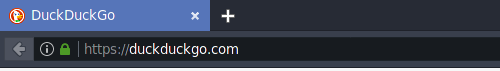
\includegraphics[scale=1]{Duck.png}\\
		\footnotesize O cadeado verde representa o certificado SSL
	\end{center}

	O certificado SSL nem sempre está nos sites, principalmente em sites pequenos, é comum eles não terem um certificado SSL. Mas caso aconteça de algum site importante, como o site do Facebook ou o site do teu banco não tenha certíficado SSL, é recomendável não fazer login.\\

\pagebreak

	Os \href{https://criptowiki.miraheze.org/wiki/Spam}{spams} foram um método muito utilizado como forma de espalhar malwares e também para poder fazer phishing em usuários.\\

	Os spams são basicamente mensagens enviada para e-mails aleatórios com algum link para o usuário acessar ou algum arquivo para baixar. Eles foram e ainda são bem comuns, embora não seja um método muito eficaz atualmente, mas caso receba alguma mensagem por e-mail com um título sensacionalista, é recomendável não abri-lo. Então a dica é que antes de abrir uma mensagem de e-mail, pense 2 vezes ao abri-lo e se abrir, pense bem antes de clicar em algo.\\

	Os arquivos e programas que são baixados na internet, muitas vezes podem vir com algum software malicioso junto ao arquivo ou programa baixado, desta forma, dando ao invasor total controle da máquina. Se for baixar algum arquivo ou software, certifique-se que ele está sendo baixado do site oficial ou até mesmo pela loja de software do sistema operacional.\\

\pagebreak

\section*{Navegadores, Cookies, Trackers e muito mais}
	"\textbf{\textit{Data is money, my friend}}", sim, dados são dinheiro e empresas tem os dados de bilhões de usuários em todo o mundo.\\

	Com a popularização da internet, o uso de navegadores é muito comum entre usuários em todo o mundo, mas enquanto usuários navegam na internet utilizando navegadores, correm um grande risco e podem perder a privacidade.\\

\subsection{Cookies}
	Os \textbf{\textit{cookies}} são pequenos pacotes de dados enviados de um site para o navegador (\textit{browser}) do usuário, para que possa guardar informações do usuário, como login e senha, itens adicionado no carrinho de compras de lojas online e outras informações.\\

	Os cookies são um grande risco à privacidade de usuários, por que eles vem ativos por padrão no browser e vários sites utilizam cookies de outros sites para poderem obter informações do usuário.\\

\subsection{Trackers}
	Os \textbf{\textit{trackers}} são scripts que tem como objetivo monitorar os usuários, coletando informações de cookies da página para que possam capturar dados para fazerem propagandas direcionadas. Os trackers estão incluidos na grande maioria das páginas web existentes atualmente. É estimado que 10\% de toda os sites da web tem trackers do \textbf{\textit{Google}}, \textbf{\textit{Facebook}} e \textbf{\textit{Twitter}}. Os trackers, em sua maioria faz sincronização de cookies, comunicando a outros trackers os ID's usados internamente para identificar visitantes.\\

	Os trackers, por serem quase que onipresentes na web, eles coletam e compartilham informações entre si e assim criar um perfil sobre o usuário.\\

\footnote{\href{https://antivigilancia.org/pt/2015/11/trackers-os-grandes-stalkers-da-web/}{Trackers: Os grandes stalkers da web}}

\subsection{Por que eles querem os dados dos usuários?}
	Atualmente, informação é o que move a economia digital, através da coleta de dados de bilhões de usuários no mundo, empresas se mantem, trocando serviços "\textit{gratuitos} e recebem em troca os dados dos usuários que utilizam os serviços. Empresas como \textbf{\textit{Google}} e \textbf{\textit{Facebook}}, tem uma quantidade gigantesca de dados de \textbf{\textit{bilhões}} de usuários e simplesmten os vendem para quem deseja usa-los.\\

	\begin{center} % Insere uma imagem.
		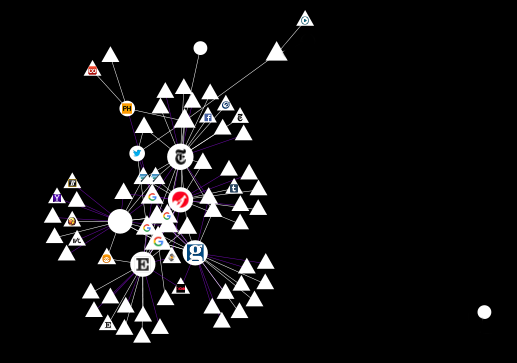
\includegraphics[scale=0.7]{trackers1.png}\\
		\footnotesize Trackers de sites. O ponto isolado é o WikiLeaks.
	\end{center}


	Esses dados possuem alto valor para uma série de outras empresas que se beneficiam em conhecer detalhes sobre a vida das pessoas: serviços de crédito que querem avaliar seu risco de dar um calote, seguros de saúde que podem usá-los para determinar o valor do plano, lojas e empreendimentos que querem entender o comportamento do mercado e anunciar diretamente para um público-alvo específico.\\

\footnote{\href{https://antivigilancia.org/pt/2016/06/webcensus/}{Estudo de Princeton expõe vigilância descontrolada dos trackers na Web}}
\footnote{\href{https://antivigilancia.org/pt/2015/05/data-brokers-e-profiling-um-guia-ilustrado/}{Data Brokers e Profiling: um guia ilustrado}}

	Por este mercado ser tão grande, surgiram empresas que vendem dados de usuários, estas empresas são chamadas de \textit{data brockers}, uma gigante deste ramo, a \textbf{\textit{Experian}}, que em seus bancos de dados possuem informações de populações inteiras e que possuem \textit{terabytes} de informações sobre a população brasileira e \textit{petabytes} de informações à nível global.\\

	\begin{center}
		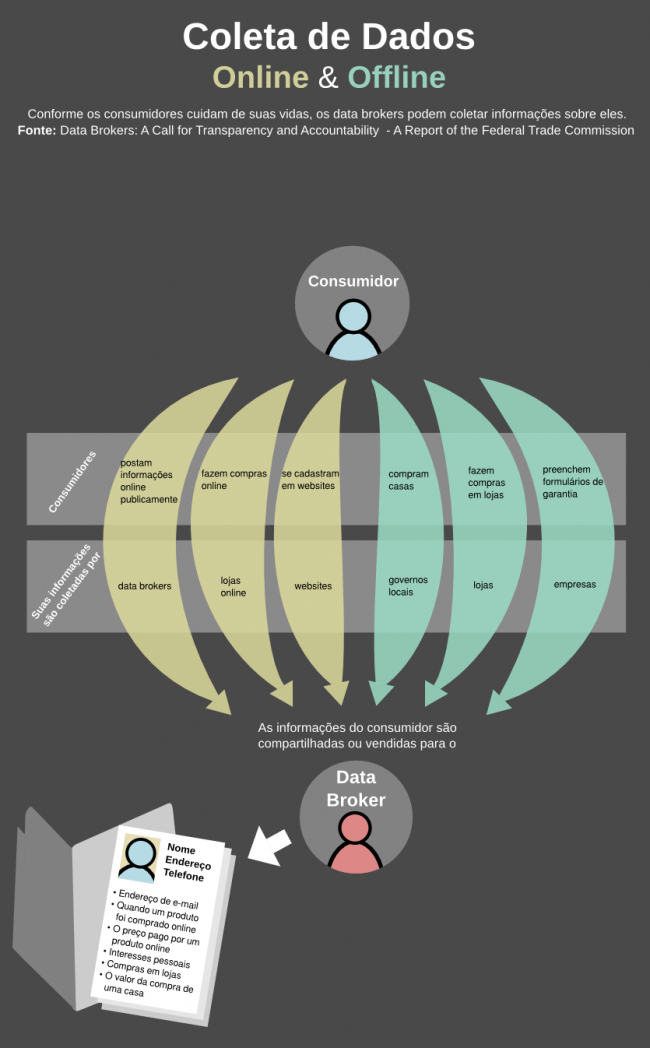
\includegraphics[scale=0.60]{databrokers.png}\\
		\footnotesize Tradução do infográfico produzido pela Federal Trade Commission dos Estados Unidos em sua análise sobre a a atualização dos data brokers. Feito para o artigo Data Brokers e Profiling: vigilância como modelo de negócios.
	\end{center}

\subsection{Como se proteger?}
	Felizmente, existem alguns softwares que os usuários podem utilizar para que diminua esta vigilância em massa feita por empresas, estes softwares tentam bloquear anúncios e trackers. O \textit{AdBlock} e \textit{Privacy Badger}, que são extenções de navegador que tentam bloquear anúncios e trackers.\\

	Softwares como o \href{https://linuxroot1.github.io/DNSCRYPT-Proxy/}{DNSCrypt-Proxy} também tentam bloquear malwares, anúncios e trackers à nível de DNS.\\

	Para usuários que se preocupam mais com a privacidade, existe a extensão \textbf{\textit{NoScript}} que bloqueia todos os scripts JavaScript por padrão e também o \textbf{\textit{uMatrix}}, que permite selecionar com ainda mais precisão com que tipo de funcionalidades pode interagir.



\section*{Senhas - O elo mais fraco da nossa segurança}

As senhas são certamente uma das partes mais importantes da segurança e da privacidade. Com as senhas dos usuários na mão de pessoas mal intencionadas, pode-se fazer um grande estrago aos usuários. Embora as senhas sejam tão importantes para a segurança, ainda assim a maioria dos usuários espalhados pelo mundo usam senhas fracas e que comprometem a segurança dos usuários.\\

\subsection{Por que nossas senhas não são boas?}

\begin{itemize}
	\item Viés cognitivo: as pessoas tem uma intuição deturpada de resultado aleatório, onde certas sequencias são favorecidas, esse comportamento de manada acaba produzindo senhas mais previsíveis.
	\item Intuitivamente acreditamos que senha boa é uma senha complicada e super difícil de lembrar, quando na realidade para computadores são super fáceis de serem quebradas.
	\item Exemplo: "\textit{S\&nha5F0d@}", tem 9 caracteres (contendo maiúsculas, minúsculas, números e caracteres especiais), mas é quebrada em segundos.
\end{itemize}

	Pelas senhas serem tão frágeis, devemos ter senhas boas, mas então temos uma questão, \textit{como podemos ter senhas boas?}\\

\subsection{Como gerar boas senhas? Método Diceware}

	O método \textit{diceware} é um método no qual, através de um dado, uma lista de palavras mais papel e lápis, podemos construir senhas mais seguras.\\

	O método consiste em usar o dado para sortear palavras da lista. Jogue o dado 5 vezes por palavra. Os dois primeiros números são as páginas do livreto e os três últimos a palavra.\\

	\textbf{Exemplo}: O usuário jogou o dado 5 vezes, tirando os números: \textbf{\textit{2-6-5-1-3}}. O usuário deverá ir até a página 2 e 6 do livreto e procurar pela palavra \textbf{\textit{513}}, que será "\textbf{\textit{egípcio}}.\\

	É recomendado usar no mínimo 6 palavras utilizando o método do \textit{diceware}.\\


	\footnote{Consulte o \href{https://github.com/thoughtworks/dadoware}{livreto} da ThoughtWorks para poder pegar a lista de palavras.}


\subsection{Aprimorando o Diceware}

	Para podermos gerar senhas ainda mais seguras utilizando o diceware, podemos:

\begin{itemize}
	\item Colocar alguns caracteres especiais e números entre as palavras.
	\item Colocar aleatoriamente algumas letras em maiúsculas.
	\item Utilizar termos técnicos e palavras que não existem em dicionários e listas.\\
\end{itemize}

	Em suma, o Diceware é um método de gerar senhas que é:

\begin{itemize}
	\item Harder: As senhas geradas são verdadeiramente aleatórias, as tornando bem mais difíceis de quebrar.
	\item Better: São melhores para lembrar.
	\item Faster: É mais rápido de de pensar numa senha, basta jogar o dado (ou fazer no computador).
	\item Stronger: As senhas geradas são mais fortes, pois tem muito mais combinações.
\end{itemize}

	\footnote{Gerador de senha utilizando o método Diceware: \href{https://github.com/caioau/personal/blob/master/DicewareGen/dicewareGen.py}{Diceware Generetor}}.

\subsection{Geradores de senhas (Password Manager)}

	Os password manager's são uma boa ferramenta para que usuários possam gerar senhas aleatórias e gerenciá-las de uma forma fácil.\\

	Password managers são programas que criam boas senhas aleatórias automaticamente, para cada site individualmente, guardando todas essas senhas trancadas com apenas uma senha mestra.\\

	O \textbf{KeePassX} é uma boa recomendação para usuários poderem gerenciar senhas de forma segurança, além de ele ser um software livre e que está disponível para várias plataformas, como Windows, Android, distribuições Linux entre outros sistemas.\\

	O uso do \textbf{KeePassX} é simples: o usuário cria o seu banco de senhas (\textit{.kdb ou .kdbx}), cadastra as entradas dos serviços usados e, então, o programa gera uma senha aleatória.\\
	Quando o usuário precisar acessar uma senha, terá de abrir o arquivo, digitar a senha mestra e então selecionar a entrada que precisa.\\

\begin{itemize}
	\item Control+c: Copia a senha.
	\item Control+b: Copia o usuário.
\end{itemize}

\pagebreak

% DNS
\section*{DNS}
	O \href{https://criptowiki.miraheze.org/wiki/DNS_(Domain_Name_System)}{DNS} (\textbf{Domain Name System}) é o responsável por levar o usuário até o site desejado.\\
	Suponha-se que o usuário deseja ir até o site \textbf{google.com}, para que ele possa ir até o site, é necessário ir até o \href{https://pt.wikipedia.org/wiki/IP}{IP} correspondente do site. O DNS é o responsável por levar o usuário até o IP correspondente ao site.
	O servidor DNS interfere e muito na velocidade da conexão e também é possível que o servidor DNS seja invadido por alguém mal intencionado e utilizar o servidor DNS para que possa fazer um ataque phishing e assim fazer todos os usuários que utilizam aquele servidor acreditar que o site que está sendo acessado é o verdadeiro, quando na verdade é um site falso.\\

	No terceiro dia de 2017, houve um caso de invasão de servidores DNS e o site do Google aparecia com uma imagem diferente:

\begin{center} % Insere uma imagem.
	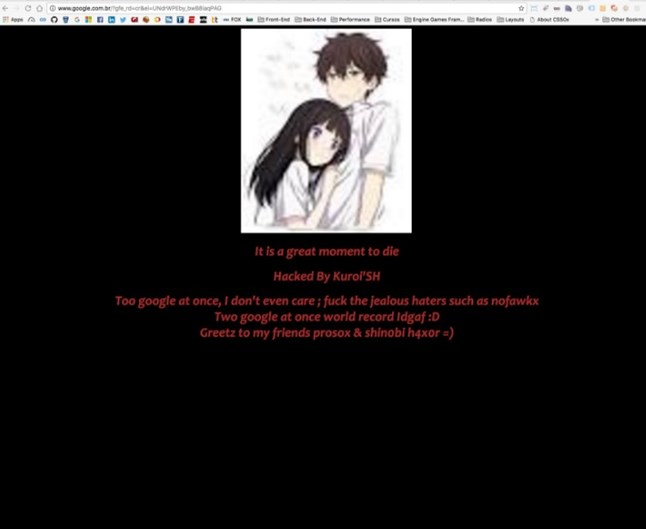
\includegraphics[scale=0.7]{dns.jpg}\\
\end{center}

	Geralmente, usuários não configuram o servidor DNS que será utilizado pelo sistema e por padrão, o sistema utiliza o servidor DNS oferecido pelo próprio provedor de internet, o que pode não ser uma boa ideia visto que ISP (Internet Service Provider) pode ser infectado fácilmente e que ele não é especializado nisto.\\


	Existem diversos servidores DNS seguros e que são recomendados e utilizados por técnicos em segurança.\\

	Servidores DNS recomendados:

	\begin{itemize} % Inicia uma lista.
		\item OpenDNS
		\item Google DNS
		\item DynDNS
		% \item texto_aqui... É para inserir um novo objeto à lista.
%
	\end{itemize} % Termina a lista.

	Para poder configurar o servidor DNS que será utilizado é bastante simples e por isto não irei demonstrar aqui, basta uma rápida pesquisa em algum site de busca para que você possa encontrar tutoriais.\\

\pagebreak

% Segurança nos sistemas operacionais.
\section*{Segurança nos sistemas operacionais}
	O sistema operacional (\textbf{OS}) é a parte mais importante de um computador. É onde tudo ocorre, é onde o usuário usa a internet, edita documentos, guarda documentos e várias outras atividades e é exatamente por isto que deve-se mantê-lo seguro e livre de ameaças.\\

	O sistema operacional para computadores mais utilizados atualmente é o Windows. Embora o Windows seja considerado por muitos como o melhor sistema operacional, na realidade não é bem assim. O Windows é um sistema operacional totalmente fechado, que quer dizer que nenhuma linha de código do sistema está exposto para que o usuário possa ver. Por este motivo, caso a Microsfot  deseje, ela pode colocar algum \href{https://criptowiki.miraheze.org/wiki/Backdoors}{backdoor} no OS e assim, não apenas a Microsoft mas também qualquer pessoa mal intencionada poderia fazer uso deste backdoor para poder controlar a máquina e roubar dados do usuário.\\

	Além do Windows ser um sistema fechado, ele também tem diversas vulnerabilidades e que não são exploradas apenas por hackers mas também por governos, como é o caso dos recentes vazamentos de ferramentas que eram utilizadas pela NSA para poder explorar vulnerablidades no protocolo SMB do Windows. Estas ferramentas foram vazadas pelo grupo \textbf{Shadown Brokers}. Estas ferramentas foram utilizadas para criar o WannaCry que é um \href{https://criptowiki.miraheze.org/wiki/Ransomwares}{ransomware}. Este ransomware infectou milhares de máquinas em todo o mundo e gerou uma grande repercução em todo o globo pelo seu tempo de propagação que durou horas e que já tinha infectado vários países.\\

\begin{center} % Insere uma imagem.
	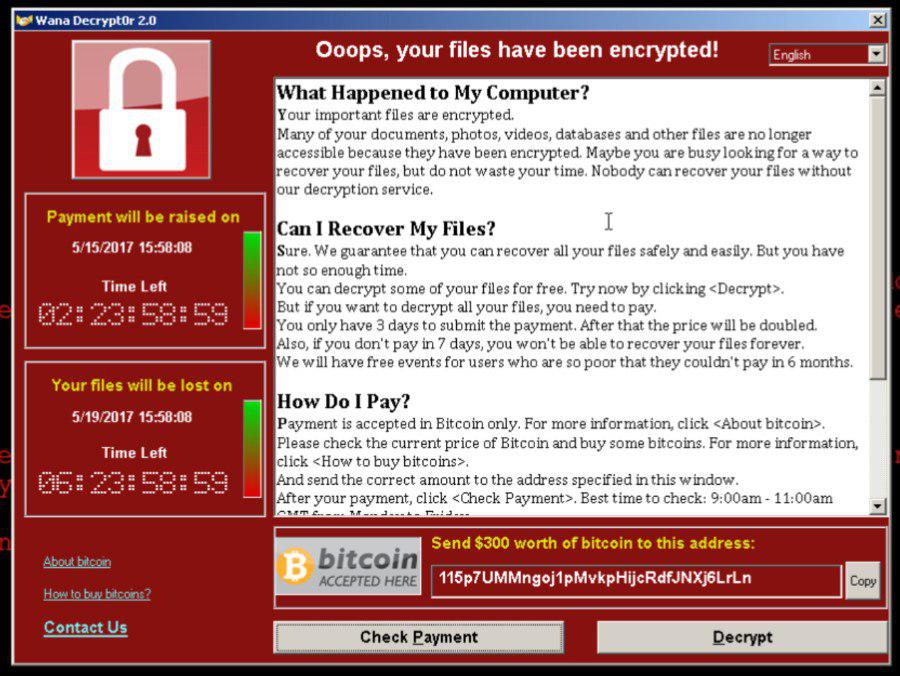
\includegraphics[scale=0.8]{wannacry.jpg}\\
	\footnotesize WannaCry % Descrição da imagem que vem logo abaixo.
\end{center}

	Além do Windows ser um OS com várias falhas, também é um sistema que "espiona" os usuários, mandando diversas informações para os servidores da Microsoft e assim corrompendo a privacidade dos usuários. Um outro ponto negativo no Windows é o tempo de correção de falhas que podem durar semanas ou até meses ({\textit alguns casos demoraram até 6 meses}), o que é extremamente ruim para os usuários que ficam vulneraveis durante meses e as ferramentas para explorar estas falhas estão na internet para que qualquer um possa utilizá-las.\\

	Em distribuições Linux, na qual o código fonte dos programas e do sistema operacional é aberto para que qualquer um possa olhar, as correções de falhas podem durar alguns dias ou ({/textbf raramente}) alguns meses. E também, distribuições Linux tem poucas falhas. Mais para frente, irei falar um pouco sobre o Linux.\\

	Em geral, existem falhas, mas ainda assim é bom o usuário ficar atento e manter o sistema seguro. As dicas dada por profissionais de segurança são:

	\begin{itemize} % Inicia uma lista.
		\item Manter o sistema atualizado.
		\item Não baixar softwares de sites não confiáveis
		\item Não baixar arquivos que não se sabe de quem ou o que é.
		\item Sempre baixar softwares dos sites ou repositórios oficiais.
		\item Usar softwares renomados e que de preferência seja OpenSource.
		\item Manter backups constantes de arquivos importantes.
	\end{itemize} % Termina uma lista.

	Estas dicas são básicas, porém é recomendado segui-las para que os usuários não sejam tão facilmente infectados por malwares.\\

\pagebreak

\part{Capítulo 2 - Segurança em nível médio.}

\section*{Engenharia Social - A falha humana na segurança}
	Uma das maiores falhas na segurança é certamente os humanos, que podem ser enganados facilmente por alguém mal intencionado. A \textbf{\textit{engenharia social}} é justamente a técnica que explora os humanos para que possa conseguir informações privilegiadas, e com as informações em mãos, conseguir fazer ataques, descobrir senhas de redes sociais, bancos e etc.\\

\subsection{O que é engenharia social}
	A engenharia social é uma técnica de manipulação psicológica de pessoas para a execução de ações ou divulgar informações confidenciais. Este tipo de ataque depende muito da interação humana para que possa quebrar procedimentos de segurança.\\
	O ser humano tem traços de comportamento e psicológicos que o tornam suscetíveis a ataques de engenharia social, como o pré-julgamento de uma pessoa por ela estar ou não bem vestida, também pelo tom de voz da pessoa e outros fatores e assim o atacante poderá obter a confiança da pessoa e consequentemente informações privilegiadas.\\

	Um dos maiores hackers que já existiu, \textbf{\textit{Kevin Mitnick}}, usou diversas vezes a engenharia social para que pudesse conseguir informações privilegiadas para que pudesse invadir sistemas telefônicos.\\

	A engenharia é o método mais rápido e eficaz para que se possa invadir sistemas, pois os humanos são falhos e facilmente enganados. A engenharia social não é apenas usado físicamente, mas também na internet, como é o caso dos spams que usam a engenharia social para poder infectar pessoas.\\

\subsection{Se protegendo da engenharia social}
	A engenharia social faz uso da ingenuidade (\textit{ou burrice}) das pessoas para poder obter informações privilegiadas. E como para a ingenuidade não existe remédio, a engenharia social continuará sendo eficaz, mas existem dicas para que não seja tão fácil cair em engenharia social na internet:

\begin{itemize}
	\item Não confiar em qualquer pesquisa que peça dados pessoais.
	\item Não fornecer senhas por meios eletrônicos. (Telefone, e-mail, mensageiros e etc)
	\item Não acreditar em tudo que chega pelo e-mail.
	\item Não confiar em redes sem fios (WiFi) abertas.
	\item Não abrir arquivos de fontes não oficiais.
	\item Não pensar que estes tipos de ataques acontecem apenas com outras pessoas.
	\item Não confiar muito nas pessoas.
	\item Sempre desconfiar das pessoas.
\end{itemize}

	Estas dicas são bastante simples, mas podem salvar diversos usuários simplesmente por seguir estas dicas básicas. Então, nunca confie muito nas pessoas e nem deem dados importantes, como data de nascimento, nome, número de telefone e outras informações pessoais.\\

\pagebreak

\section*{Smartphones e a segurança digital}
	Por smartphones serem baratos e de fácil uso, nos últimos anos, eles se popularizaram bastante e se tornou o meio de acesso à internet mais utilizado em todo o planeta. Mas por smartphones serem tão utilizados, os criminosos passaram a focar os seus esforços para atacar vítimas que utilizam os smartphones.\\

\subsection{Os riscos}
	Nesta era de informação, "tudo" está conectado à rede, informações podem sair da China e chegar até a cidade de São Paulo em minutos, mas por conta disso, não é apenas informações que viajam e se espalham facilmente, mas também trojans, worms, \textbf{ransomwares} e vários outros malwares.\\

	Aplicativos como o \textit{WhatsApp} são utilizado por milhões de pessoas em todo o planeta, então, qualquer um se torna um alvo em potencial. Milhões de usuários no Brasil já caíram em golpes no WhatsApp. Estas mensagens de golpes que os usuários recebem, muitas vezes são sensacionalistas, falam algo extremamente fantástico e infelizmente, por ingenuidade, alguns usuários caem nestes golpes que utilizam a \textit{engenharia social} para poderem convencer suas vítimas.\\

<<<<<<< HEAD
	Hoje em dia, pelo fácil acesso à internet, usuários que preferem não pagar por aplicativos, buscam maneiras "ilegais" para poderem ter acesso aos aplicativos, mas muitas vezes sai mais caro do que comprar os aplicativos. Quando se baixa alguma \textbf{\textit{APK}} em algum site na internet, existe uma grande chance de que esta APK venha com algum malware junto a APK, então, é sempre bom tomar cuidado ao baixar APK's de sites não oficiais e não confiáveis, \textit{pois o barato pode sair caro}.


\footnote{\href{https://www.tecmundo.com.br/whatsapp/116247-novo-golpe-whatsapp-futebol-atingiu-2-milhoes-brasileiros.htm}{Novo golpe do WhatsApp sobre futebol já atingiu 2 milhões de brasileiros}

	Hoje em dia, pelo fácil acesso à internet, usuários que preferem não pagar por aplicativos, buscam maneiras "ilegais" para poderem ter acesso aos aplicativos, mas muitas vezes sai mais caro do que comprar os aplicativos. Quando se baixa alguma \textbf{\textit{APK}} em algum site na internet, existe uma grande chance de que esta APK venha com algum malware junto a APK, então, é sempre bom tomar cuidado ao baixar APK's de sites não oficiais e não confiáveis, \textit{pois o barato pode sair caro}.\\

	Não é apenas com golpes do WhatsApp e malwares passado através de APK's de aplicativos que os usuários devem se preocupar. Redes wireless (\textit{WiFi}) nos dias atuais tem se tornado populares e quase que em qualquer lugar se encontra alguma rede wireless e algumas vezes, se encontra hotspots públicos para que a população use-os. Mas os usuários devem ficar atentos à rede que eles se conectam, pois podem ser vítimas de um ataque MITM (\textit{Man In The Midle}). O recente vazamento do \textbf{\textit{WikiLeaks}}, nomeado de \href{https://wikileaks.org/vault7/#Cherry\%20Blossom}{Cherry Blossom}, que faz parte da série de vazamentos do \textit{\textbf{Vault7}}, mostra que a CIA estava utilizando um sistema de hacking para redes wireless. O \textbf{\textit{Charry Blossom}} monitorava redes wirelles, inclusive redes públicas e podiam fazer ataques MITM, controlando o trafego dos alvos para qualquer lugar.\\


\footnote{\href{https://www.tecmundo.com.br/whatsapp/116247-novo-golpe-whatsapp-futebol-atingiu-2-milhoes-brasileiros.htm}{Novo golpe do WhatsApp sobre futebol já atingiu 2 milhões de brasileiros}}

\end{document} % Fim do documento.
